\subsection{Proposed workaround}

%
In the first proposed approach, blocks are characterized using a failure criteria on the output.
If the output goes beyond this criteria, the failure duration is recorded.
The characterization is done with a large range of input amplitude and duration.
This yiels a large 2D table that associates to an input amplitude and input duration, an output duration.
This table is a part of the block model.
The output amplitude must also be modeled to be able to predict the output waveform from the input waveform.
Since the characterization is performed with a fixed failure criteria, almost all information regarding the output amplitude is lost.
The only remaining data is whether the criteria was violated or not.
It was supposed earlier that this limitation is the main source of error.

% What is kept in the method, What is modified
A modification of the characterization method is proposed.
The failure criteria on the output is removed.
Instead, the extreme output amplitude value is recorded in addition to the duration.
The block model now contains two 2D tables instead of one.
The first table still associates an output duration to an input width/amplitude.
The second and new table associates an output amplitude to an input width/amplitude.

Fig. \ref{fig:principle-transfert-func-v2} summarizes the new model.
Function $F_{W}$ uses the first table mentioned previously.
It returns for an arbitrary input amplitude and width the closest output width found in the table.
Function $F_{V}$ is identical, except it is using the second table, and returns the closest output amplitude.

\begin{figure}[!h]
  \centering
  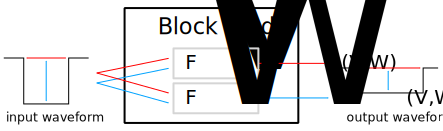
\includegraphics{src/4/figures/principle_transfert_function_v2.pdf}
  \caption{Improved modelling method}
  \label{fig:principle-transfert-func-v2}
\end{figure}

% What's the global idea, hypothesis here
The method described here relies on the hypothesis that the entire top-level circuit is not required for ESD simulations.
The behavior of the block could be reproduced with a decent accuracy in the condition that it is correctly biased and loaded.
Under those conditions the output is supposed to vary similarly between a full simulation and a light, single-block simulation.
Of course, to obtain the response of multiple blocks, models must be connected or chained together.
Fig. \ref{fig:full-method-v2} illustrates the entire characterization and chaining process.

\begin{figure}[!hp]
  \centering
  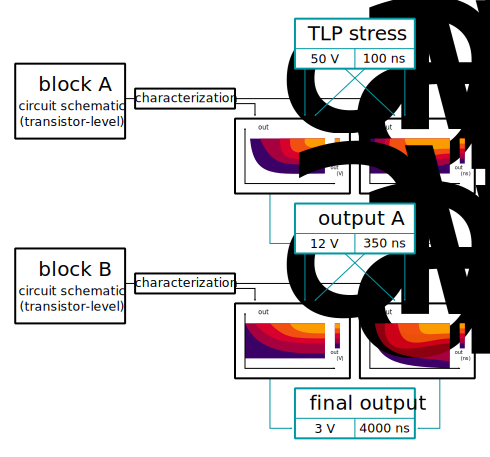
\includegraphics[width=0.7\textwidth]{src/4/figures/full_method_overview_v2.pdf}
  \caption{Overview of improved bottom-up method - example with two blocks}
  \label{fig:full-method-v2}
\end{figure}

\subsubsection{Preliminary application}
% First run the reference sim
To test this new approach, a few simulations are run.
A first reference simulation is performed first.
It contains the complete schematic, composed of the three blocks of our study case.
An electrical disturbance is injected on the first input $V_{batt}$.
The final output $V_{2p5}$, and intermediate nets $V_{clamp9}$ and $V_{1p0}$ are observed and disturbance properties on those nets recorded.

%TODO: Schema setups

% Then do the same thing but with the individual models
Afterwards, each block is simulated separately in its own testbench.
The first block is stressed with the same pulse than the reference simulation.
Its output waveform is compared with the reference in Fig. \ref{fig:sim-compare-block1}.
Both curves (blue and green) look rather similar, in terms of maximum amplitude, duration and overall shape.
The maximum amplitude is estimated at -1.5 V and the duration at 880 ns.
The red curve represents the waveform injected on the second block and configured using these two values.

\begin{figure}[!h]
  \centering
  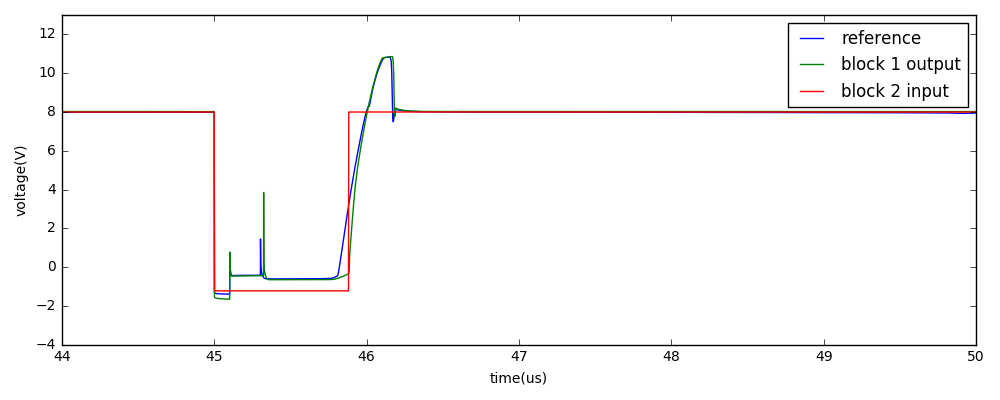
\includegraphics[width=0.98\textwidth]{src/4/figures/simulation_comparison_block1.png}
  \caption{$V_{clamp9}$ waveform}
  \label{fig:sim-compare-block1}
\end{figure}

% Second block output
On the second block output, the blue and green waveforms exhibit more differences (Fig. \ref{fig:sim-compare-block2}).
The green waveform has a longer slope than the reference.
However, both waveforms are still quite close in terms of maximum amplitude and duration.
This is an interesting results, because it shows that blocks can be simulated individually for ESD waveforms, without loosing too much accuracy.
This is great for simulation speed and modularity.
Once again, the red curve represents the waveform injected on the third block.
It is a simplified waveform derived from the blue and green curves, with a width of 2 \textmugreek{}s and an amplitude of 0V.

\begin{figure}[!h]
  \centering
  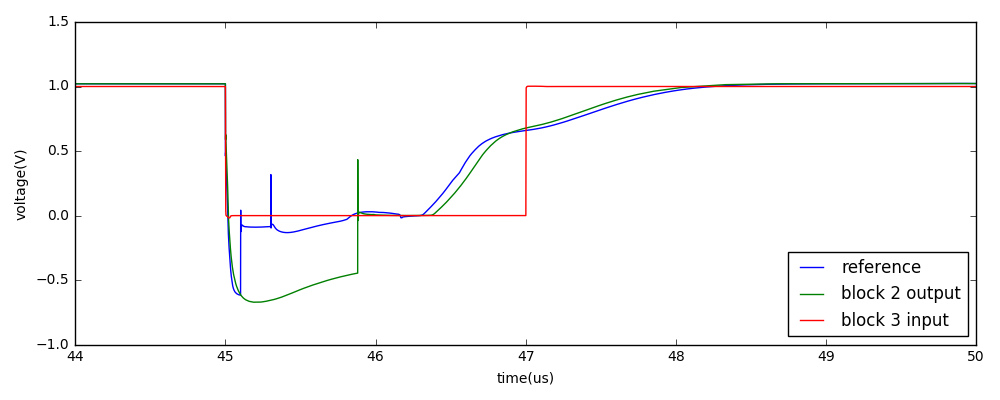
\includegraphics[width=0.98\textwidth]{src/4/figures/simulation_comparison_block2.png}
  \caption{$V_{1p0}$ waveform}
  \label{fig:sim-compare-block2}
\end{figure}

% Third output
On the third and final block output (Fig. \ref{fig:sim-compare-block3}), both waveforms are very similar.
The difference in terms of maximum amplitude can be explained by an offset between both curves a $t=0$.
The reference curve is delayed in comparison of the individual simulation, but otherwise both curves match.

\begin{figure}[!h]
  \centering
  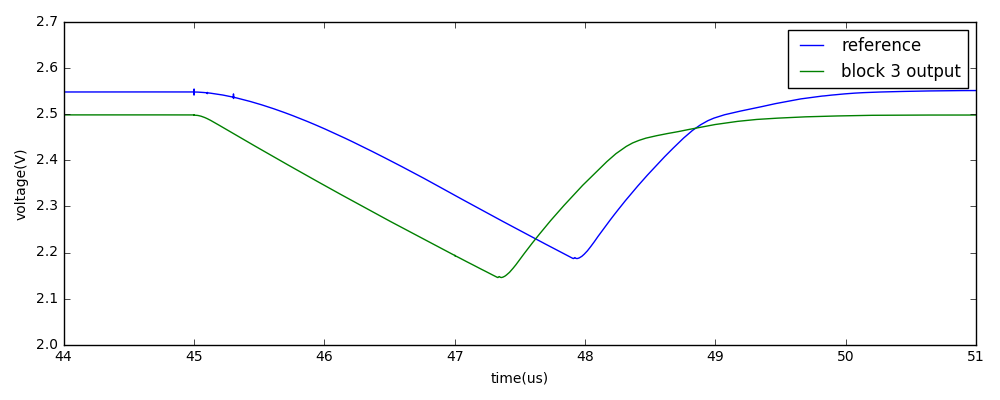
\includegraphics[width=0.98\textwidth]{src/4/figures/simulation_comparison_block3.png}
  \caption{$V_{2p5}$ waveform}
  \label{fig:sim-compare-block3}
\end{figure}

% Conclusion, it works for this case
In conclusion, for this specific study-case, simulating the models isolately produced the same results than the reference simulation, for estimating degradation of functionality.
The consequence is that block models extracted from variable amplitude/width characterization should work properly, since it is mathematically equivalent to the simulations that were performed in this section (block models can be seen as pre-computed simulations).

The next section discusses how to automate the extraction of a width and amplitude from a waveform, in order to simplify it.

\subsubsection{Automating model extraction}

% What is the challenge regarding the extraction of the models
In the simulations described earlier, a single width and maximum amplitude per waveform were extracted manually.
However, the waveforms are not square at all, and an width and amplitude cannot always be extracted easily.
The challenge is to find the right rule for simplifying them into a rectangular waveform, and extracting the two parameters.
This applies to the input waveform, and the output waveform.

% First approach with a 90% amplitude
Initially, the rules were to set $V$ equal to the maximum value of the waveform (input or output), and $W$ the width of the pulse at 90\% of $V$.
The concept is illustrated in Fig. \ref{fig:impact-single-failure-criteria} with a few example curves.

\begin{figure}[!h]
  \centering
  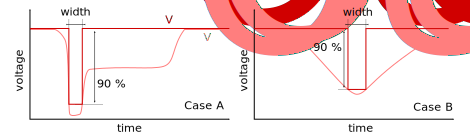
\includegraphics[width=0.98\textwidth]{src/4/figures/better_output_modelling.pdf}
  \caption{Improved output modelling method based on 90\% of maximum disturbance amplitude}
  \label{fig:impact-single-failure-criteria}
\end{figure}

% Problems with the 90% threshold
In case \textit{A}, the waveform can be simplified easily into a rectangular pulse.
However, this 90\% threshold does not work reliably with cases \textit{B} and \textit{C}.

% Explain case B
Case \textit{B} is often observed during the injection of an electrostatic discharge.
The \gls{esd} signal is superimposed on top of a slow signal variation.
In that case, the waveform exhibits a very short, high amplitude peak, followed by slower smaller-amplitude variation.
The width of the pulse is much shorter than the original curve, leading the model to be very inaccurate.

% Explain case C
Case \textit{C} is observed on nets with high capacitive coupling to ground.
Those signals are not directly disturbed by the \gls{esd}, but the block that drives them can go into reset.
In this situation, the nets slowly decreases then, once functionnality resumes, the nets goes back to its nominal value.
With the 90\% threshold, a large area of the disturbed waveform is missing in the model, making it very inaccurate.

% What is the consequence
In both those cases, the 90\% threshold leads to underestimating the total disturbance width.
The modeled waveform has a much smaller duration and area than the original one.
Overall, it was observed that the model and original waveform areas should be close for the models to work.

% The relative threshold is not good enough, a smarter technique is required
Instead of focusing on the peak amplitude, a smarter method is required.
Ideally, it needs to extract a width and amplitude that would result in the same area than the original waveform, while looking as similar as possible.

%TODO
A feature detection method using amplitude distribution could be performed to identify key amplitudes in the waveforms.

\subsection{Limitations, conclusion and follow-up work}

% Sum up what was done
Laid ground principles for an operating ESD block modeling method.
Started from W&B method, based on a pass/fail failure criteria.
Method was improved to fit better analog functions modeling.
Main concept is to simplify waveforms to turn them into a rectangular shape.
Then, simple characterization tables can represent the impact of any block on a waveform.
First tests are quite successfull.
On a single study-case, it was shown that this method works for predicting the failure of an output given an input stress.

%TODO: Review
Ultimately, the goal is to build a simpler representation of the output waveform of a block, composed of square shapes.
The main advantage of those shape is that they are understood by the block models.
It could be seen as a mathematical transformation of a time-domain waveform into a square-domain waveform.

% Limitations
How to handle real circuit topology (interconnect mesh) versus the linear one used in the characterization.
Talk about 1 pin to many pin that is ok, but many pin to 1 is not covered at all by this method
Talk about ESAAS, electrical simulations as a service, as an alternative to black-box block models

% Conclusion

% Follow up work
Make more study cases, validate on more circuits and blocks
